\documentclass[10pt,c,aspectratio=1610,handout]{beamer}
\usetheme[block=fill,numbering=fraction,progressbar=frametitle]{metropolis}
%\usecolortheme{beaver}
\usepackage{textpos}
\usepackage{amsmath}
\usepackage{amssymb}
\usepackage{appendixnumberbeamer}

\setbeamercovered{transparent}

\newcommand\blfootnote[1]{%
  \begingroup
  \renewcommand\thefootnote{}\footnote{#1}%
  \addtocounter{footnote}{-1}%
  \endgroup
}

\renewcommand{\baselinestretch}{1.25}
% Colour theme
\definecolor{QDMblue}{rgb}{0.00, 0.1882, 0.3608}
\definecolor{QDMgold}{rgb}{0.9098, 0.6510, 0.0000}
\definecolor{QDMgreen}{rgb}{0.3098, 0.5490, 0.0510}
\setbeamercolor{normal text}{ fg= QDMblue , bg= white }
\setbeamercolor{alerted text}{ fg= QDMgold }
\setbeamercolor{example text}{ fg= QDMgreen }

\begin{document}

% Personal Info
\title{Lecture 06: Solving for the Dynamics of a DSGE Model}%
\author[Konstantin Gantert]{\begin{large} Konstantin Gantert \end{large} \\ \textbf{Quantitative Dynamic Macroeconomics}}
\date{\textit{this version:} \today}%

% Eliminates Navigation Bar on every Frame
\beamertemplatenavigationsymbolsempty%

%-------------------------------------------------------------------------
% 0.1 Titlepage
%-------------------------------------------------------------------------
{\setbeamertemplate{footline}{}%
\frame{\titlepage}}%
 \addtocounter{framenumber}{-1}%
%-------------------------------------------------------------------------
% ABOUT THE LECTURE
%-------------------------------------------------------------------------
% Outline for this Lecture
\begin{frame}{Outline for this Lecture}%
  \onslide<1->{%
    \begin{minipage}{0.48\textwidth}%
      \textbf{What have we seen so far}%
      \begin{enumerate}%
        \item A model of money and capital {\tiny [CG 1, 5]}%
        \item Equilibrium tax distortions {\tiny [CG 5, 6]}%
        \item Optimal labor \& capital taxation {\tiny [CG 3, 6]}%
      \end{enumerate}%
    \end{minipage}%
  }%
  \hfill%
  \onslide<3->{%
    \begin{minipage}{0.48\textwidth}%
      \textbf{What we will see today}%
      \begin{enumerate}%
        \item Stochastic CiA model with capital {\tiny [CG 1, 5]}%
        \item State-space and recursive methods {\tiny [CG 1, 5]}%
        \item Approximation \& undet. coeff. {\tiny [CG 3, 4]}%
        \item Calibration \& quantitative analysis {\tiny [CG 4, 5]}%
      \end{enumerate}%
    \end{minipage}%
  }%
  \vspace*{0.25in}%
  \onslide<2->{%
    \begin{block}{Big Picture of the Lecture:}%
      \begin{enumerate}%
        \item How can we solve intertemporal dynamic models?%
        \item What role do random shocks play in the solution?%
      \end{enumerate}%
    \end{block}%
  }%
\end{frame}%
%-------------------------------------------------------------------------
% BLOCK 1: The Complete CiA Dynamic Stochastic General Equilibrium Model
%-------------------------------------------------------------------------
\section{The Complete CiA Dynamic Stochastic General Equilibrium Model}%
%-------------------------------------------------------------------------
% The Household Utility Maximization Problem
\begin{frame}{The Household Utility Maximization Problem}%
  Each household maximizes utility by choosing $\{ C_t, L_t, M_{t+1}, B_{t+1}, K_{t+1} \}_{t=1,2}$ such that%
  \begin{align*}%
    \max \; \mathbb{E}_t \left\{ \sum_{t=1,2} \beta^{t-1} \left[ u(C_t) - v(L_t) \right] + \beta^2 \mathbb{V} \left(M_3,B_3,K_3\right) \right\}%
  \end{align*}%
  subject to%
  \begin{align*}%
    M_t \; \geq \; P_t C_t%
  \end{align*}%
  \pause%
  \begin{align*}%
    & P_t \left[ \left(Z_t L_t\right)^{1-\alpha} K_t^\alpha - \delta K_t \right] + \left[ M_t - P_t C_t \right] + B_t + T_t\\%
    & \geq \; M_{t+1} + q_t B_{t+1} + P_t \left[ K_{t+1} - K_t \right] \quad \forall t \leq 2%
  \end{align*}%
\end{frame}%
%-------------------------------------------------------------------------
% Model Setup
\begin{frame}{Model Setup: First-Order Conditions}%
  The model is solved by its \textbf{FOCs and constraints} as follows:%
  \begin{align}%
    1 \; = & \;\tilde{\lambda}_t + \tilde{\mu}_t\\%
    \tilde{\mu}_t \; = & \; \frac{\beta}{1+\tau_t}\\%
    L_t^{\gamma} \; = & \; \frac{\beta}{\left(1+\tau_t\right) C_t} Z_t^{1-\alpha} \left(1-\alpha\right) L_t^{-\alpha} K_t^{\alpha}\\%
    1 \; = & \; \mathbb{E}_t \left[ \frac{\beta\left(1+\tau_t\right)C_t}{\left(1+\tau_{t+1}\right)C_{t+1}} \left[ \left(Z_{t+1}L_{t+1}\right)^{1-\alpha} \alpha K_{t+1}^{\alpha-1} + 1 - \delta \right] \right]\label{eq:foc_capital}\\%
    C_t \; = & \; \left(Z_t L_t\right)^{1-\alpha} K_t^\alpha + (1-\delta) K_t - K_{t+1}%
  \end{align}%
  \vspace*{-0.2in}%
  \pause%
  \begin{itemize}%
    \item[$\blacktriangleright$] We use a change-in-variables as in previous lectures to derive the above conditions.%
    \item[$\blacktriangleright$] The first two FOCs are determined only by parameters and exogenous variables, hence we can substitute them out in the last three equations.%
    \item[$\blacktriangleright$] \alert{\textbf{Be mindful about the expectations operator in (\ref{eq:foc_capital})!}}%
  \end{itemize}%
\end{frame}%
%-------------------------------------------------------------------------
% Model Setup: Fixed-Point Representation
\begin{frame}{Model Setup: Fixed-Point Representation}%
  Therefore, the three-equation block of the model that solves for the equilibrium is given by:%
  \begin{align}%
    F^L(\cdot) \; = & \; L_t^{\gamma} - \frac{\beta}{\left(1+\tau_t\right) C_t} Z_t^{1-\alpha} \left(1-\alpha\right) L_t^{-\alpha} K_t^{\alpha} \; = \; 0\label{eq:foc_labor}\\%
    F^K(\cdot) \; = & \; 1 - \mathbb{E}_t \left[ \frac{\beta\left(1+\tau_t\right)C_t}{\left(1+\tau_{t+1}\right)C_{t+1}} \left[ \left(Z_{t+1}L_{t+1}\right)^{1-\alpha} \alpha K_{t+1}^{\alpha-1} + 1 - \delta \right] \right] \; = \; 0\\%
    F^C(\cdot) \; = & \; C_t - \left(Z_t L_t\right)^{1-\alpha} K_t^\alpha - (1-\delta) K_t + K_{t+1} \; = \; 0\label{eq:foc_consumption}%
  \end{align}%
  \begin{itemize}%
    \item[$\blacktriangleright$] (\ref{eq:foc_labor})-(\ref{eq:foc_consumption}) completely describes the model dynamics.%
    \item[$\blacktriangleright$] The labor and consumption conditions depend only on current values.%
    \item[$\blacktriangleright$] But the capital conditions has a much richer pattern of dependence.%
    \pause%
    \item[$\Rightarrow$] \textbf{Issue of Solving the Model:} We are seeking a sequence of functions $\{ C_t, L_t, K_{t+1} \}_{t=1}^{\infty}(s_t)$ that satisfy these three conditions at each point in time.%
  \end{itemize}%
\end{frame}%
%-------------------------------------------------------------------------
% BLOCK 2: State Space Form and Recursive Methods
%-------------------------------------------------------------------------
\section{State Space Form\\and Recursive Methods}%
%-------------------------------------------------------------------------
% DSGE Models from a Mathematical Point of View
\begin{frame}%
  \frametitle{DSGE Models from a Mathematical Point of View}%
  Any DSGE model can be represented by a function%
  \begin{align*}%
    f \left(X, U\right) \quad = \quad 0,%
  \end{align*}\\%
  \vspace*{-0.1in}%
  where %
  \begin{itemize}%
    \item[$\blacktriangleright$] $X$ is a $N\;x\;T$ matrix with $N$ endogenous variables across $T$ periods,%
    \item[$\blacktriangleright$] $U$ is a $M\;x\;T$ matrix with $M$ exogenous variables across $T$ periods.%
  \end{itemize}%
  \pause%
  A model can have%
  \begin{itemize}%
    \item[$\blacktriangleright$] a finite number of endogenous variables, $N$, and exogenous variables, $M$,%
    \item[$\blacktriangleright$] many periods, $t = 0,1,2, ..., T$, with possibly $T \rightarrow \infty$,%
    \item[$\blacktriangleright$] many (possibly infinitely many) histories, $U_0, U_1, ..., U_t$.%
  \end{itemize}%
  \vspace*{0.1in}%
  \pause%
  \textbf{Main Issue:} We have to solve for a potentially very large number of unknowns!%
\end{frame}%
%-------------------------------------------------------------------------
% Determining the Size of the Model
\begin{frame}%
  \frametitle{Determining the Size of the Model}%
  \begin{block}{Size of the Problem:}%
    \vspace*{-0.1in}%
    \begin{align*}%
      \left( \# Variables, \quad \# Periods, \quad \# Histories \right)%
    \end{align*}%
    \vspace*{-0.2in}%
  \end{block}%
  \pause%
  \begin{itemize}%
    \item[$\blacktriangleright$] \textbf{No Uncertainty and Finite Number of Periods}%
    \begin{itemize}%
      \item[$\rightarrow$] $N\;x\;T\;x\;1$ unknowns: Relatively small problem to solve!%
      \item[$\rightarrow$] Solve for $N\;x\;T$ (non-linear) equations and unknowns.%
      \item[$\rightarrow$] See two-period model in assignment 0.%
    \end{itemize}%
    \pause%
    \item[$\blacktriangleright$] \textbf{No Uncertainty and Infinite Number of Periods}%
    \begin{itemize}%
      \item[$\rightarrow$] $N\;x\;\infty\;x\;1$ unknowns: Impossible to solve!%
      \item[$\rightarrow$] Well approximated by a large number of periods.%
      \item[$\rightarrow$] See e.g. Cole (2020) chapter 19.4: Shooting algorithm.%
    \end{itemize}%
    \pause%
    \item[$\blacktriangleright$] \textbf{Uncertainty and Infinite Number of Periods}%
    \begin{itemize}%
      \item[$\rightarrow$] $N\;x\;\infty\;x\;\infty$ unknowns: Impossible to solve!%
      \item[$\rightarrow$] Approximation requires large number of periods for every history (also a large number).%
      \item[$\rightarrow$] Hence, difficult to solve! \textbf{\alert{Possible Solution?}} $\Rightarrow$ Recursive Methods and Approximation!%
    \end{itemize}%
  \end{itemize}%
  \vspace*{-0.1in}%
\end{frame}%
%-------------------------------------------------------------------------
% Recursive Methods and the Policy Function (1/2)
\begin{frame}%
  \frametitle{Recursive Methods and the Policy Function (1/2)}%
  \begin{itemize}%
    \item[$\blacktriangleright$] \textbf{Main Idea:} Break the model into smaller pieces (state-space form):%
      \begin{align*}%
        \mathbb{E}_t f \left(X_{t-1},X_t,X_{t+1},U_t,U_{t+1}\right) \quad = \quad 0%
      \end{align*}%
      \vspace*{-0.2in}%
      \begin{footnotesize}%
        \begin{itemize}%
          \item[$\blacktriangleright$] $\mathbb{E}_t$ is a rational expectation operator, $X_t$ is a vector of model variables, and $U_t$ is a vector of exogenous shocks.%
          \item[$\blacktriangleright$] Decisions at any point in time depend on the state of the economy, $X_{t-1}$, the exogenous shocks, $U_t$, and the expectation about the future, $\left(\mathbb{E}_t X_{t+1}; \mathbb{E}_t U_{t+1}\right)$.%
        \end{itemize}%
      \end{footnotesize}%
      \pause%
    \item[$\blacktriangleright$] Variables in period $t$ depend only on the variables fully describing the history:%
      \begin{align*}%
        X_t \quad = g \left(X_{t-1},U_t\right),%
      \end{align*}%
      where $g\left(.\right)$ is a vector of unknown functions \emph{(constant across time)}.%
      \pause%
      \vspace*{0.1in}%
    \item[$\Rightarrow$] Hence, instead of solving for $\{X_t\}_{t=0}^{\infty}$, solve for a \textbf{vector of policy functions}, $\{ g\left(.\right) \}_{n=1}^{N}$!%
  \end{itemize}%
\end{frame}%
%-------------------------------------------------------------------------
% Recursive Methods and the Policy Function (2/2)
\begin{frame}%
  \frametitle{Recursive Methods and the Policy Function (2/2)}%
  \begin{block}{The Model in State-Space Form with Policy Functions:}%
    \vspace*{-0.1in}%
    \begin{align*}%
      \mathbb{E}_t f \left(X_{t-1},g\left(X_{t-1},U_t\right),g\left(g\left(X_{t-1},U_t\right),U_{t+1}\right),U_t,U_{t+1}\right) \quad = \quad 0%
    \end{align*}%
  \end{block}%
  \pause%
  \begin{footnotesize}%
    \textbf{Example - apply it to our model (see (\ref{eq:foc_labor})-(\ref{eq:foc_consumption})):}%
    \begin{align}%
      F^L(\cdot) \; = & \; (g_{L_t})^{\gamma} - \frac{\beta}{\left(1+\tau_t\right) (g_{C_t})} Z_t^{1-\alpha} \left(1-\alpha\right) (g_{L_t})^{-\alpha} (g_{K_t})^{\alpha} \; = \; 0\\%
      F^K(\cdot) \; = & \; 1 - \mathbb{E}_t \left[ \frac{\beta\left(1+\tau_t\right)(g_{C_t})}{\left(1+\tau_{t+1}\right)(g_{C_{t+1}})} \left[ \left(Z_{t+1}(g_{L_{t+1}})\right)^{1-\alpha} \alpha (g_{K_{t+1}})^{\alpha-1} + 1 - \delta \right] \right] \; = \; 0\\%
      F^C(\cdot) \; = & \; (g_{C_t}) - \left(Z_t (g_{L_t})\right)^{1-\alpha} K_t^\alpha - (1-\delta) K_t + (g_{K_{t+1}}) \; = \; 0%
    \end{align}%
    \pause%
    where%
    \begin{align*}%
      L_t:= & \quad g_{L_t} \; = \; g_L \left(s_t\right) \; = \; g_L \left( K_t, Z_t, \tau_t \right)\\%
      C_t:= & \quad g_{C_t} \; = \; g_C \left(s_t\right) \; = \; g_C \left( K_t, Z_t, \tau_t \right)\\%
      K_{t+1}:= & \quad g_{K_{t+1}} \; = \; g_K \left\{s_t\right\} \; = \; g_K \left( K_t, Z_t, \tau_t \right)\\%
      \pause%
      L_{t+1}:= & \quad g_{L_{t+1}} \; = \; g_L \left(s_{t+1}(s_t)\right) \; = \; g_L \left(K_{t+1},Z_{t+1},\tau_{t+1}\right) \; = \; g_L \left(g_K \left( K_t, Z_t, \tau_t \right),Z_{t+1},\tau_{t+1}\right)\\%
      C_{t+1}:= & \quad  g_{C_{t+1}} \; = \; g_C \left(s_{t+1}(s_t)\right) \; = \; g_C \left(K_{t+1},Z_{t+1},\tau_{t+1}\right) \; = \; g_C \left(g_K \left( K_t, Z_t, \tau_t \right),Z_{t+1},\tau_{t+1}\right)%
    \end{align*}%
    \vspace*{-0.2in}%
    \pause%
    \begin{itemize}%
      \item[$\rightarrow$] We still need to define processes for the exogenous variables/shocks (e.g. AR(1))!%
    \end{itemize}%
  \end{footnotesize}%
\end{frame}%
%-------------------------------------------------------------------------
% Solving for the Policy Function
\begin{frame}%
  \frametitle{Solving for the Policy Function}%
  How can we solve for the \textbf{policy functions} of the model economy?%
  \begin{itemize}%
    \item[$\blacktriangleright$] The policy function is a largely unknown function for us.%
    \item[$\blacktriangleright$] It is a solution to system of (non-linear) first-order difference equations.%
  \end{itemize}%
  \pause%
  In this course: \textbf{Perturbation Method!} It requires 3 steps:%
  \begin{enumerate}%
    \item Calculating the \textbf{deterministic steady-state}:%
    \begin{footnotesize}%
    \begin{itemize}%
      \item[$\rightarrow$] Known point of the system of first-order difference equations:\\%
      \textbf{Deterministic Steady-State:} $f\left(\bar{X},\bar{X},\bar{X},0,0\right)=0$.%
    \end{itemize}%
    \end{footnotesize}%
    \pause%
    \item \textbf{Approximating} the dynamic system of equations:%
    \begin{footnotesize}%
    \begin{itemize}%
      \item[$\rightarrow$] Approximation works well for small deviations around the deterministic steady-state.%
      \item[$\rightarrow$] It relies on the differentiability of the system of equations.%
      \item[$\rightarrow$] It can easily handle very large economic systems.%
    \end{itemize}%
    \pause%
    \end{footnotesize}%
    \item \textbf{Solving} for the first-order system of difference equations:%
    \begin{footnotesize}%
    \begin{itemize}%
      \item[$\rightarrow$] Method of Undetermined Coefficients%
    \end{itemize}%
    \end{footnotesize}%
  \end{enumerate}%
\end{frame}%
%-------------------------------------------------------------------------
% BLOCK 3: Taylor Approximation: Linearization of the System of Equations
%-------------------------------------------------------------------------
\section{Taylor Approximation:\\{\normalsize Linearization of the System of Equations}}%
%-------------------------------------------------------------------------
% First-Order Taylor Approximation (1/2)
\begin{frame}%
  \frametitle{First-Order Taylor Approximation (1/2)}%
  \begin{block}{Definition}%
    \begin{align*}%
      f\left(x,y\right) \quad \approx \quad f\left(x_0,y_0\right) + \frac{\partial f\left(x_0,y_0\right)}{\partial x} \left(x_t - x_0\right) + \frac{\partial f\left(x_0,y_0\right)}{\partial y}\left(y_t-y_0\right)%
    \end{align*}%
  \end{block}%
  \pause%
  \begin{itemize}%
    \item[$\blacktriangleright$] Given is the following equation $f \left(x,y\right) = g \left(x,y\right)$.%
    \item[$\blacktriangleright$] Its steady-state is given by $f \left(x_0,y_0\right) = g \left(x_0,y_0\right)$.%
    \pause%
    \item[$\blacktriangleright$] We calculate the Taylor approximation of both sides according to%
    \begin{align*}%
      &\frac{\partial g\left(x_0,y_0\right)}{\partial x} \left(x_t - x_0\right) + \frac{\partial g\left(x_0,y_0\right)}{\partial y}\left(y_t-y_0\right)\\%
      & \quad \approx \frac{\partial f\left(x_0,y_0\right)}{\partial x} \left(x_t - x_0\right) + \frac{\partial f\left(x_0,y_0\right)}{\partial y}\left(y_t-y_0\right),%
    \end{align*}%
    where the steady-state on both sides cancels out.%
  \end{itemize}%
\end{frame}%
%-------------------------------------------------------------------------
% First-Order Taylor Approximation (2/2)
\begin{frame}%
  \frametitle{First-Order Taylor Approximation (2/2)}%
  In order to calculate percentage deviations from the steady-state, we use%
  \begin{align*}%
    \hat{x}_t \quad = \quad \frac{x_t-x_0}{x_0},%
  \end{align*}%
  and plug it into the Taylor approximation%
  \begin{align*}%
    \frac{\partial g\left(x_0,y_0\right)}{\partial x} x_0 \hat{x}_t + \frac{\partial g\left(x_0,y_0\right)}{\partial y}y_0 \hat{y}_t \approx \frac{\partial f\left(x_0,y_0\right)}{\partial x} x_0 \hat{x}_t + \frac{\partial f\left(x_0,y_0\right)}{\partial y}y_0 \hat{y}_t.%
  \end{align*}\\%
  \pause%
  \vspace*{0.2in}%
  \textbf{Certainty Equivalence:}%
  \begin{itemize}%
    \item[$\blacktriangleright$] The following condition holds in linear models: $\mathbb{E} \left[f\left(X\right)\right] = f\left(\mathbb{E}\left[X\right]\right)$.%
    \item[$\blacktriangleright$] Only first moments (expected values) matter for the decisions.%
    \item[$\blacktriangleright$] Expectations play no role in linear models: \textbf{Certainty Equivalence}!%
  \end{itemize}%
\end{frame}%
%-------------------------------------------------------------------------
% Nth-Order Taylor Approximation
\begin{frame}%
  \frametitle{Nth-Order Taylor Approximation}%
  \begin{block}{Definition}%
    \begin{align}%
      \begin{split}%
        f\left(x\right) \quad \approx & \quad f\left(x_0\right) + \frac{f'\left(x_0\right)}{1!} \left(x_t-x_0\right) + \frac{f''\left(x_0\right)}{2!} \left(x_t-x_0\right)^2\\%
        & \quad + \frac{f'''\left(x_0\right)}{3!} \left(x_t-x_0\right)^3 + \dots + \frac{f^N\left(x_0\right)}{N!} \left(x_t-x_0\right)^N%
      \end{split}%
    \end{align}%
  \end{block}%
  \pause%
  We need at least ...%
  \begin{itemize}%
    \item[$\blacktriangleright$] a second-order Taylor approximation to include (constant) uncertainty in the model.%
    \item[$\blacktriangleright$] a third-order Taylor approximation to include conditional uncertainty in the model.%
  \end{itemize}%
  \vspace*{0.15in}%
  We can completely approximate any equation of order N by a Nth-order Taylor approximation.%
\end{frame}%
%-------------------------------------------------------------------------
% What Degree of Approximation to Choose?
\begin{frame}%
  \frametitle{What Degree of Approximation to Choose?}%
  \begin{figure}%
    \centering%
    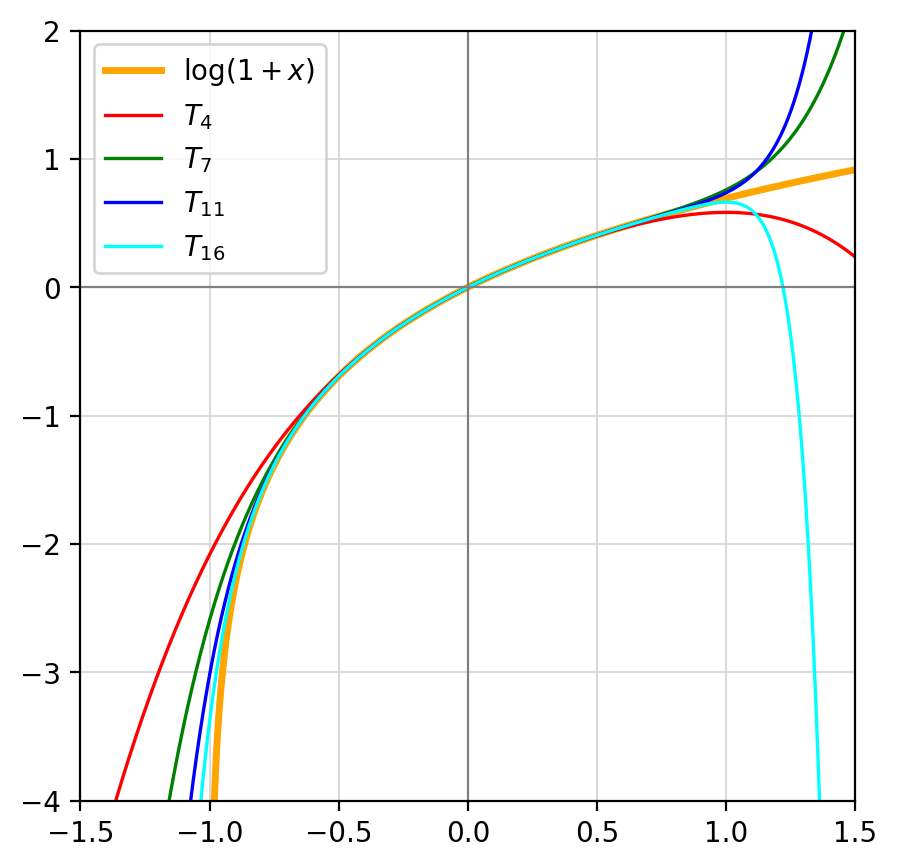
\includegraphics[width=0.5\textwidth]{figures/taylor_approx_order.png}\\%
    {\scriptsize Taylor polynomials of order 4, 7, 11 and 16 of $\log(1+x)$ around $x=0$ (own illustration).}%
  \end{figure}%
  \vspace*{-0.1in}%
  \begin{itemize}%
    \item[$\Rightarrow$] The function fit of the approximation does \textbf{NOT} increase monotonically in the order of the approximation!%
  \end{itemize}%
\end{frame}%
%-------------------------------------------------------------------------
% Example: Linearization of our CiA DSGE Model (1/3)
\begin{frame}%
  \frametitle{Example: Linearization of our CiA DSGE Model (1/3)}%
  \textbf{Capital Law of Motion}%
  \begin{itemize}%
    \item[$\blacktriangleright$] Original Equation:%
      \begin{align*}%
        K_{t+1} \quad = \quad \left(1-\delta\right) K_{t} + X_t%
      \end{align*}\\%
    \vspace*{-0.1in}%
    \pause%
    \item[$\blacktriangleright$] Steady-State:%
      \begin{align*}%
        X \quad = \quad \delta K%
      \end{align*}\\%
    \vspace*{-0.1in}%
    \pause%
    \item[$\blacktriangleright$] Linearized Equation:%
    \begin{align*}%
      \left(K_{t+1}-K\right) \quad = & \quad \left(1-\delta\right) \left(K_{t}-K\right) + \left(X_t - X\right)\\%
      \pause%
      K \frac{K_{t+1}-K}{K} \quad = & \quad \left(1-\delta\right) K \frac{K_{t}-K}{K} + X \frac{X_t-X}{X}\\%
      \pause%
      K \hat{K}_{t+1} \quad = & \quad \left(1-\delta\right) K \hat{K}_{t} + X \hat{X}_t\\%
      \pause%
      \hat{K}_{t+1} \quad = & \quad \left(1-\delta\right) \hat{K}_{t} + \frac{X}{K} \hat{X}_t\\%
      \pause%
      \hat{K}_{t+1} \quad = & \quad \left(1-\delta\right) \hat{K}_{t} + \delta \hat{X}_t%
    \end{align*}%
  \end{itemize}%
\end{frame}%
%-------------------------------------------------------------------------
% Example: Linearization of our CiA DSGE Model (2/3)
\begin{frame}%
  \frametitle{Example: Linearization of our CiA DSGE Model (2/3)}%
  \textbf{Production Function}%
  \begin{itemize}%
    \item[$\blacktriangleright$] Original Equation:%
      \begin{align*}%
        Y_t \quad = \quad Z_t K_{t}^\alpha L_t^{1-\alpha}%
      \end{align*}\\%
    \vspace*{-0.1in}%
    \pause%
    \item[$\blacktriangleright$] Steady-State:%
      \begin{align*}%
        Y \quad = \quad Z K^\alpha L^{1-\alpha}%
      \end{align*}\\%
    \vspace*{-0.1in}%
    \pause%
    \item[$\blacktriangleright$] Linearized Equation:%
      \begin{align*}%
        \left(Y_t-Y\right) \quad = & \quad K^\alpha L^{1-\alpha} \left(Z_t-Z\right) + Z K^{\alpha-1} L^{1-\alpha} \alpha \left(K_{t}-K\right)\\%
        & \quad + Z K^\alpha L^{-\alpha} \left(1-\alpha\right) \left(L_t-L\right)\\%
        \pause%
        Y \frac{Y_t-Y}{Y} \quad = & \quad Z K^\alpha L^{1-\alpha} \left[\frac{Z_t-Z}{Z} + \alpha \frac{K_{t}-K}{K}+ \left(1-\alpha\right)\frac{L_t-L}{L}\right]\\%
        \pause%
        Y \hat{Y}_t \quad = & \quad Z K^\alpha L^{1-\alpha} \left[\hat{Z}_t + \alpha \hat{K}_{t}+ \left(1-\alpha\right) \hat{L}_t\right]\\%
        \pause%
        \hat{Y}_t \quad = & \quad \hat{Z}_t + \alpha \hat{K}_{t} + \left(1-\alpha\right) \hat{L}_t%
      \end{align*}%
  \end{itemize}%
\end{frame}%
%-------------------------------------------------------------------------
% Example: Linearization of our CiA DSGE Model (3/3)
\begin{frame}%
  \frametitle{Example: Linearization of our CiA DSGE Model (3/3)}%
  \textbf{Linearized CiA DSGE Model}%
  \vspace*{0.2in}%
  \begin{align}%
    F^L(\cdot) \; = & \; \left(\gamma+\alpha\right) \hat{L}_t - \left[ (1-\alpha) \hat{Z}_t + \alpha \hat{K}_t - \hat{C}_t - \hat{\tau}_t \right] \; = \; 0\\%
    \notag\\%
    F^K(\cdot) \; = & \; \mathbb{E}_t \hat{C}_{t+1} - \hat{C}_t - \hat{\tau}_t + \mathbb{E}_t \hat{\tau}_{t+1} - \Sigma_1 \mathbb{E}_t \left[ \hat{Z}_{t+1} + \hat{L}_{t+1} - \hat{K}_{t+1} \right] \; = \; 0\\%
    \notag\\%
    F^C(\cdot) \; = & \; \hat{C}_t - \left(1+\delta \Sigma_2\right) \left[ (1-\alpha) \left(\hat{Z}_t+\hat{L}_t\right) + \alpha \hat{K}_t \right] - \Sigma_2 \left[ (1-\delta)\hat{K}_t - \mathbb{E}_t \hat{K}_{t+1} \right] \; = \; 0%
  \end{align}%
  where%
  \begin{align*}
    \Sigma_1 \; = & \; \left(1-\beta(1-\delta)\right) (1-\alpha)\\%
    \Sigma_2 \; = & \; \frac{\alpha}{\frac{1-\beta}{\beta}+\delta(1-\alpha)}%
  \end{align*}
\end{frame}%
%-------------------------------------------------------------------------
% BLOCK 4: Method of Undetermined Coefficients
%-------------------------------------------------------------------------
\section{Method of Undetermined Coefficients}%
%-------------------------------------------------------------------------
% Setup of the Method of Undetermined Coefficients (1/2)
\begin{frame}%
  \frametitle{Setup of the Method of Undetermined Coefficients (1/2)}%
  \textbf{Solution Approach:}%
  \begin{itemize}%
    \item[$\blacktriangleright$] Take a \textbf{''guess''} of the solution of the system of difference equations.%
    \item[$\blacktriangleright$] The solution must be \textbf{linear}, since the model is linear.%
    \item[$\blacktriangleright$] Each \textbf{decision} on the control variables is based on state and exogenous stock variables.%
    \pause%
    \item[$\blacktriangleright$] A guess to the solution takes the form%
      \begin{align}%
        \hat{L}_t \; = \; g_L \left(\hat{K}_t, \hat{Z}_{t}, \hat{\tau}_t\right) \; = & \;  \psi_{L,K} \hat{K}_{t} + \psi_{L,Z} \hat{Z}_{t} + \psi_{L,\tau} \hat{\tau}_{t} \\%
        \hat{C}_t \; = \; g_C \left(\hat{K}_t, \hat{Z}_{t}, \hat{\tau}_t\right) \; = & \; \psi_{C,K} \hat{K}_{t} + \psi_{C,Z} \hat{Z}_{t} + \psi_{C,\tau} \hat{\tau}_{t} \\%
        \hat{K}_{t+1} \; = \; g_K \left(\hat{K}_t, \hat{Z}_{t}, \hat{\tau}_t\right) \; = & \; \psi_{K,K} \hat{K}_{t} + \psi_{K,Z} \hat{Z}_{t} + \psi_{K,\tau} \hat{\tau}_{t}%
      \end{align}%
      where $\psi_{L,K}, \psi_{L,Z}, \psi_{L,\tau}, \psi_{C,K}, \psi_{C,Z}, \psi_{C,\tau}, \psi_{K,K}, \psi_{K,Z}$, and $\psi_{K,\tau}$ are the \textbf{undetermined coefficients}. They depend on the parameters of the model (educated guess).%
  \end{itemize}%
\end{frame}%
%-------------------------------------------------------------------------
% Setup of the Method of Undetermined Coefficients (2/2)
\begin{frame}%
  \frametitle{Setup of the Method of Undetermined Coefficients (2/2)}%
  \textbf{Expectations about future variables} {\small(symmetric for other variables and shock processes)}:%
  \begin{align}%
    \mathbb{E}_t \hat{Z}_{t+1} \quad = & \quad \mathbb{E}_t \left( \rho_Z \hat{Z}_t + \epsilon_{Z,t+1}\right) \quad = \quad \rho_Z \hat{Z}_t\\
    \pause%
    \mathbb{E}_t \hat{C}_{t+1} \quad = & \quad \mathbb{E}_t \left[ \psi_{C,K} \hat{K}_{t+1} + \psi_{C,Z} \hat{Z}_{t+1} + \psi_{C,\tau} \hat{\tau}_{t+1}\right]\notag\\%
    \pause%
    = & \quad \psi_{C,K} \left( \psi_{K,K} \hat{K}_{t} + \psi_{K,Z} \hat{Z}_{t} + \psi_{K,\tau} \hat{\tau}_{t} \right)\notag\\%
    & \quad + \psi_{C,Z} \rho_{Z} \hat{Z}_t + \mathbb{E}_t \hat{\epsilon}_{Z,t+1} + \psi_{C,\tau} \rho_\tau \hat{\tau}_t + \mathbb{E}_t \hat{\epsilon}_{\tau,t+1}\notag\\%
    \pause%
    = & \quad \psi_{C,K} \left( \psi_{K,K} \hat{K}_{t} + \psi_{K,Z} \hat{Z}_{t} + \psi_{K,\tau} \hat{\tau}_{t} \right) + \psi_{C,Z} \rho_{Z} \hat{Z}_t + \psi_{C,\tau} \rho_\tau \hat{\tau}_t%
  \end{align}%
  \pause%
  \begin{small}%
    \begin{itemize}%
      \item[$\blacktriangleright$] \textbf{Constant policy functions:} Future decisions are made the same way as today, given expectations of future states and exogenous variables.%
      \item[$\blacktriangleright$] \textbf{Iterative approach:} Expected future state variables are set by the decisions today.%
      \item[$\blacktriangleright$] \textbf{Certainty Equivalence:} Only first moments (expected values) are part of the policy functions.%
      \item[$\blacktriangleright$] \textbf{Uncertainty} (second moments) does not play any role!%
    \end{itemize}%
  \end{small}%
\end{frame}%
%-------------------------------------------------------------------------
% Solving for the Undetermined Coefficients (1/5)
\begin{frame}%
  \frametitle{Solving for the Undetermined Coefficients (1/5)}%
  Substitute the policy functions for the (expected) control variables in the reduced-form model. The \textbf{labor FOC} is given by:%
  \begin{footnotesize}%
    \begin{align*}%
      \begin{split}%
        F^L(\cdot) \; = & \; \left(\gamma+\alpha\right) \left[ \psi_{L,K}\hat{K}_t + \psi_{L,Z} \hat{Z}_{t} + \psi_{L,\tau} \hat{\tau}_{t} \right]\\%
        & \; + \left[ \psi_{C,K} \hat{K}_t + \psi_{C,Z} \hat{Z}_{t} + \psi_{C,\tau} \hat{\tau}_{t} \right]\\%
        & \; - \alpha \hat{K}_t - \left(1-\alpha\right) \hat{Z}_t - \hat{\tau}_t \; = \; 0%
      \end{split}%
  \end{align*}%
  \end{footnotesize}%
  \pause%
  \textbf{Ordering the terms:}%
  \begin{footnotesize}%
    \begin{align}%
      \begin{split}%
        & \hat{K}_t \left[ \left(\gamma+\alpha\right) \psi_{L,K} + \psi_{C,K} - \alpha \right]\\%
         + & \hat{Z}_{t} \left[ \left(\gamma+\alpha\right) \psi_{L,Z} + \psi_{C,Z} - \left(1-\alpha\right) \right]\\%
         + & \hat{\tau}_{t} \left[ \left(\gamma+\alpha\right) \psi_{L,\tau} + \psi_{C,\tau} - 1 \right] \quad = \quad 0%
      \end{split}\label{eq:euler_policy}%
    \end{align}%
  \end{footnotesize}%
\end{frame}%
%-------------------------------------------------------------------------
% Solving for the Undetermined Coefficients (2/5)
\begin{frame}%
  \frametitle{Solving for the Undetermined Coefficients (2/5)}%
  Substitute the policy functions for the (expected) control variables in the reduced-form model. The \textbf{capital FOC} is given by:%
  \begin{footnotesize}%
    \begin{align*}%
      \begin{split}%
        F^K(\cdot) \; = & \; \left[ \psi_{C,K} \left( \psi_{K,K} \hat{K}_t + \psi_{K,Z} \hat{Z}_{t} + \psi_{K,\tau} \hat{\tau}_{t} \right) + \psi_{C,Z} \mathbb{E}_t \hat{Z}_{t+1} + \psi_{C,\tau} \mathbb{E}_t \hat{\tau}_{t+1} \right]\\%
        & \; - \left[ \psi_{C,K} \hat{K}_t + \psi_{C,Z} \hat{Z}_{t} + \psi_{C,\tau} \hat{\tau}_{t} \right] - \hat{\tau}_t + \mathbb{E}_t \hat{\tau}_{t+1}\\%
        & \; - \Sigma_1 \left[ \mathbb{E}_t \hat{Z}_{t+1} + \psi_{L,K} \left( \psi_{K,K} \hat{K}_t + \psi_{K,Z} \hat{Z}_{t} + \psi_{K,\tau} \hat{\tau}_{t} \right) + \psi_{L,Z} \mathbb{E}_t \hat{Z}_{t+1} + \psi_{L,\tau} \mathbb{E}_t \hat{\tau}_{t+1} \right.\\%
        & \; \left. \quad \quad \quad - \psi_{K,K} \hat{K}_t - \psi_{K,Z} \hat{Z}_{t} - \psi_{K,\tau} \hat{\tau}_{t} \right] \quad = \quad 0%
      \end{split}%
    \end{align*}%
  \end{footnotesize}%
  \pause%
  \textbf{Ordering the terms:}%
  \begin{footnotesize}%
  \begin{align}%
    \begin{split}%
      & \hat{K}_t \left[ \psi_{C,K} \left( \psi_{K,K} - 1 \right) - \Sigma_1 \left( \psi_{L,K} - 1 \right) \psi_{K,K} \right]\\%
      + & \hat{Z}_{t} \left[ \psi_{C,K} \psi_{K,Z} - \psi_{C,Z} - \Sigma_1 \left(\psi_{L,K} \psi_{K,Z} - \psi_{K,Z} \right) \right] + \mathbb{E}_t \hat{Z}_{t+1} \left[\psi_{C,Z} - \Sigma_1 \left(1+\psi_{L,Z}\right) \right]\\%
      + & \hat{\tau}_{t} \left[ \psi_{C,K} \psi_{K,\tau} - \psi_{C,\tau} - 1 - \Sigma_1 \left( \psi_{L,K} \psi_{K,\tau} - \psi_{K,\tau} \right) \right] + \mathbb{E}_t \hat{\tau}_{t+1} \left[ \psi_{C,\tau} + 1 - \Sigma_1 \psi_{L,\tau} \right] \quad = \quad 0%
    \end{split}\\%
    \notag\\%
    \pause%
    \begin{split}%
      \Leftrightarrow \quad & \hat{K}_t \left[ \psi_{C,K} \left( \psi_{K,K} - 1 \right) - \Sigma_1 \left( \psi_{L,K} - 1 \right) \psi_{K,K} \right]\\%
      + & \hat{Z}_{t} \left[ \psi_{C,K} \psi_{K,Z} - \psi_{C,Z} - \Sigma_1 \left(\psi_{L,K} \psi_{K,Z} - \psi_{K,Z} \right) + \rho_Z \left(\psi_{C,Z} - \Sigma_1 \left(1+\psi_{L,Z}\right) \right) \right]\\%
      + & \hat{\tau}_{t} \left[ \psi_{C,K} \psi_{K,\tau} - \psi_{C,\tau} - 1 - \Sigma_1 \left( \psi_{L,K} \psi_{K,\tau} - \psi_{K,\tau} \right) + \rho_\tau \left( \psi_{C,\tau} + 1 - \Sigma_1 \psi_{L,\tau} \right) \right] \quad = \quad 0%
    \end{split}%
  \end{align}%
  \end{footnotesize}%
\end{frame}%
%-------------------------------------------------------------------------
% Solving for the Undetermined Coefficients (3/5)
\begin{frame}%
  \frametitle{Solving for the Undetermined Coefficients (3/5)}%
  Substitute the policy functions for the (expected) control variables in the reduced-form model. The \textbf{resource constraint} is given by:%
  \begin{footnotesize}%
    \begin{align*}%
      \begin{split}%
        F^C(\cdot) \; = & \; \psi_{C,K} \hat{K}_t + \psi_{C,Z} \hat{Z}_{t} + \psi_{C,\tau} \hat{\tau}_{t} - \left(1+\delta \Sigma_2 \right) (1-\alpha) \left[ \hat{Z}_t + \psi_{L,K} \hat{K}_t + \psi_{L,Z} \hat{Z}_{t} + \psi_{L,\tau} \hat{\tau}_{t} + \frac{\alpha}{1-\alpha} \hat{K}_t \right]\\%
        & \; + \Sigma_2 \left[ \psi_{K,K} \hat{K}_t + \psi_{K,Z} \hat{Z}_{t} + \psi_{K,\tau} \hat{\tau}_{t} \right] - \Sigma_2 \left(1-\delta\right) \hat{K}_t \quad = \quad 0%
      \end{split}%
    \end{align*}%
  \end{footnotesize}%
  \pause%
  \textbf{Ordering the terms:}%
  \begin{footnotesize}%
  \begin{align}%
    \begin{split}%
      & \hat{K}_t \left[ \psi_{C,K} - \left(1+\delta \Sigma_2\right) \left[ (1-\alpha) \psi_{L,K} + \alpha \right] + \Sigma_2 \psi_{K,K} - \Sigma_2 \left(1-\delta\right) \right]\\%
      + & \hat{Z}_{t} \left[ \psi_{C,Z} - \left(1+\delta \Sigma_2\right)(1-\alpha)\left(1+\psi_{L,Z}\right) + \Sigma_2 \psi_{K,Z} \right]\\%
      + & \hat{\tau}_{t} \left[ \psi_{C,\tau} - \left(1+\delta \Sigma_2\right)(1-\alpha) \psi_{L,\tau} + \Sigma_2 \psi_{K,\tau} \right] \quad = \quad 0%
    \end{split}\label{eq:resource_policy}%
  \end{align}%
  \end{footnotesize}%
\end{frame}%
%-------------------------------------------------------------------------
% Solving for the Undetermined Coefficients (4/5)
\begin{frame}%
  \frametitle{Solving for the Undetermined Coefficients (4/5)}%
  In order for (\ref{eq:euler_policy})-(\ref{eq:resource_policy}) to hold for all possible $\hat{K}_t, \hat{Z}_{t}, \hat{\tau}_{t} \forall t$, the coefficients in the square brackets of each variable have to be zero! The following \textbf{nine conditions} are derived:%
  \begin{small}%
    \begin{align}%
      \left(\gamma+\alpha\right) \psi_{L,K} + \psi_{C,K} - \alpha \; = & \; 0\label{udc:labor_capital}\\%
      \psi_{C,K} \left( \psi_{K,K} - 1 \right) - \Sigma_1 \left( \psi_{L,K} - 1 \right) \psi_{K,K} \; = & \; 0\label{udc:capital_capital}\\%
      \psi_{C,K} - \left(1+\delta \Sigma_2\right)\left[(1-\alpha) \psi_{L,K} + \alpha\right] + \Sigma_2 \psi_{K,K} - \Sigma_2 \left(1-\delta\right) \; = & \; 0\label{udc:consumption_capital}\\%
      \pause%
      \left(\gamma+\alpha\right) \psi_{L,Z} + \psi_{C,Z} - \left(1-\alpha\right) \; = & \; 0\label{udc:labor_ar1}\\%
      \psi_{C,K} \psi_{K,Z} - \psi_{C,Z} - \Sigma_1 \left(\psi_{L,K} \psi_{K,Z} - \psi_{K,Z} \right) + \rho_Z \left(\psi_{C,Z} - \Sigma_1 \left(1+\psi_{L,Z}\right) \right) \; = & \; 0\label{udc:capital_ar1}\\%
      \psi_{C,Z} - \left(1+\delta \Sigma_2\right)(1-\alpha)\left(1+\psi_{L,Z}\right) + \Sigma_2 \psi_{K,Z} \; = & \; 0\label{udc:consumption_ar1}\\%
      \pause%
      \left(\gamma+\alpha\right) \psi_{L,\tau} + \psi_{C,\tau} - 1 \; = & \; 0\label{udc:labor_shock}\\%
      \psi_{C,K} \psi_{K,\tau} - \psi_{C,\tau} - 1 - \Sigma_1 \left( \psi_{L,K} \psi_{K,\tau} - \psi_{K,\tau} \right) + \rho_\tau \left( \psi_{C,\tau} + 1 - \Sigma_1 \psi_{L,\tau} \right) \; = & \; 0\label{udc:capital_shock}\\%
      \psi_{C,\tau} - \left(1+\delta \Sigma_2\right)(1-\alpha) \psi_{L,\tau} + \Sigma_2 \psi_{K,\tau} \; = & \; 0\label{udc:consumption_shock}%
    \end{align}%
  \end{small}%
  \vspace*{-0.2in}%
  \begin{itemize}%
    \item[$\Rightarrow$] We solve for the (non-linear) system of nine equations and nine \textbf{undetermined coefficients}, $\psi_{L,K}, \psi_{L,Z}, \psi_{L,\tau}, \psi_{C,K}, \psi_{C,Z}, \psi_{C,\tau}, \psi_{K,K}, \psi_{K,Z}$, and $\psi_{K,\tau}$!%
  \end{itemize}%
\end{frame}%
%-------------------------------------------------------------------------
% Solving for the Undetermined Coefficients (5/5)
\begin{frame}%
  \frametitle{Solving for the Undetermined Coefficients (5/5)}%
  We use (\ref{udc:labor_capital})-(\ref{udc:consumption_capital}) to solve for $\psi_{K,K}$:\\%
  {\footnotesize(it enters quadratically as we have both $K_t$ and $K_{t+1}$ as states in the policy functions)}%
  \begin{align}%
    AA \psi_{K,K}^2 + BB \psi_{K,K} + CC = 0\label{eq:coefficient_psiKK_solve}%
  \end{align}%
  where%
  \begin{scriptsize}%
    \begin{align*}%
      AA \quad = & \quad \Sigma_2 \left(\Sigma_1+\gamma+\alpha\right)\\%
      BB \quad = & \quad \left(-1\right) \left\{ \Sigma_2 \left(1-(1-\alpha)\delta\right) \left(\Sigma_1+\gamma+\alpha\right) + \Sigma_2(\gamma+\alpha) + \left(\gamma+\alpha+(1-\alpha)(1+\delta \Sigma_2)\right) \left(\Sigma_1+\alpha\right) \right\}\\%
      CC \quad = & \quad \alpha \left(\gamma+\alpha+(1-\alpha)(1+\delta \Sigma_2)\right) + \Sigma_2 \left(1-(1-\alpha)\delta\right) \left(\gamma+\alpha\right)%
    \end{align*}%
  \end{scriptsize}%
  \pause%
  It follows%
  \begin{align*}%
    \left(\psi_{K,K}\right)_{1,2} \quad = & \quad \frac{\left(-1\right)BB \pm \sqrt{BB^2 - 4 AA \cdot CC}}{2 AA}%
  \end{align*}%
\end{frame}%
%-------------------------------------------------------------------------
% Implications of $\psi_{KK}$ for Stability
\begin{frame}%
  \frametitle{Implications of $\psi_{K,K}$ for Stability}%
  There are two solutions for (\ref{eq:coefficient_psiKK_solve}). This allows for 3 different combinations:%
  \pause%
  \begin{itemize}%
    \item[$\blacktriangleright$] $\left(\psi_{K,K}\right)_1>1$ and $\left(\psi_{K,K}\right)_2>1$.\\%
      \underline{Implications:} Any exogenous shock drives $\hat{K}_t$ to $\pm \infty$. Unstable solution. $\rightarrow$ This root is ruled out by the \textbf{transversality condition!}%
      \vspace*{0.1in}%
      \pause%
    \item[$\blacktriangleright$] $\left(\psi_{K,K}\right)_1<1$ and $\left(\psi_{K,K}\right)_2<1$.\\%
      \underline{Implications:} Stable solution. But there are two stable roots for capital in the consumption policy function. This leads to no unique root and self-fulfilling expectations. $\rightarrow$ \textbf{Indeterminacy!}%
      \vspace*{0.1in}%
      \pause%
    \item[$\blacktriangleright$] $\left(\psi_{K,K}\right)_1<1$ and $\left(\psi_{K,K}\right)_2>1$.\\%
      \underline{Implications:} Stable solution. We can rule out the explosive root $\psi_{K,K}>1$. Hence, we are left with one stable root that uniquely pins down consumption (determinacy). $\rightarrow$ \textbf{Saddle-path stability!}%
  \end{itemize}%
\end{frame}%
%-------------------------------------------------------------------------
% Pinning Down the Solution
\begin{frame}%
  \frametitle{Pinning Down the Solution}%
  Given \textbf{saddle-path stability}, use the stable root to pin down the rest of the coefficients by (\ref{udc:labor_ar1}) to (\ref{udc:consumption_shock}). The policy functions give the \textbf{solution to the system of linear first-order difference equations}:%
  \begin{footnotesize}%
    \begin{align*}%
      \hat{L}_t \quad = \quad g_L \left(\hat{K}_t, \hat{Z}_{t}, \hat{\tau}_{t}\right) \quad = & \quad \psi_{L,K} \hat{K}_{t} + \psi_{L,Z} \hat{Z}_{t} + \psi_{L,\tau} \hat{\tau}_{t}\\%
      \hat{C}_t \quad = \quad g_C \left(\hat{K}_t, \hat{Z}_{t}, \hat{\tau}_{t}\right) \quad = & \quad \psi_{C,K} \hat{K}_{t} + \psi_{C,Z} \hat{Z}_{t} + \psi_{C,\tau} \hat{\tau}_{t}\\%
      \hat{K}_{t+1} \quad = \quad g_K \left(\hat{K}_t, \hat{Z}_{t}, \hat{\tau}_{t}\right) \quad = & \quad \psi_{K,K} \hat{K}_{t} + \psi_{K,Z} \hat{Z}_{t} + \psi_{K,\tau} \hat{\tau}_{t}%
    \end{align*}%
  \end{footnotesize}%
  \pause%
  The AR(1)-process of the stochastic shock is determined exogenously:%
  \begin{footnotesize}%
    \begin{align*}%
      \hat{Z}_t \quad = & \quad \rho_Z \hat{Z}_{t-1} + \hat{\epsilon}_{Z,t}\\%
      \hat{\tau}_t \quad = & \quad \rho_\tau \hat{\tau}_{t-1} + \hat{\epsilon}_{\tau,t}%
    \end{align*}%
  \end{footnotesize}%
  \pause%
  The solutions to all other variables are given by the model equations:%
  \begin{footnotesize}%
    \begin{align}%
      \hat{X}_t \quad = & \quad \frac{1}{\delta} \left( \left(\psi_{K,K} \hat{K}_{t} + \psi_{K,Z} \hat{Z}_{t} + \psi_{K,\tau} \hat{\tau}_{t} \right) - \left(1-\delta\right) \hat{K}_{t}\right)\notag\\%
      = & \quad \psi_{X,K} \hat{K}_{t} + \psi_{X,Z} \hat{Z}_{t} + \psi_{X,\tau} \hat{\tau}_{t}\\%
      \notag\\%
      \hat{Y}_t \quad = & \quad \left(1-\alpha\right) \left[ \hat{Z}_{t} + \psi_{L,K} \hat{K}_{t} + \psi_{L,Z} \hat{Z}_{t} + \psi_{L,\tau} \hat{\tau}_{t} \right] + \alpha \hat{K}_{t}\notag\\%
      = & \quad \psi_{Y,K} \hat{K}_{t} + \psi_{Y,Z} \hat{Z}_{t} + \psi_{Y,\tau} \hat{\tau}_{t}%
    \end{align}%
  \end{footnotesize}%
\end{frame}%
%-------------------------------------------------------------------------
% BLOCK 5: Calibration and Quantitative Analysis
%-------------------------------------------------------------------------
\section{Calibration\\and Quantitative Analysis}%
%-------------------------------------------------------------------------
% Calibrating the Model: Approach
\begin{frame}{Calibrating the Model: Approach}%
  \textbf{Approach to parameterize a model:}%
  \begin{itemize}%
    \item[$\blacktriangleright$] \textbf{Idea:} Set parameters of the model such that its simulation replicates aspects of the data.%
    \item[$\blacktriangleright$] \textbf{Calibration:} Set parameters according to literature, data, etc.%
    \item[$\blacktriangleright$] \textbf{Estimation:} Set parameters in an estimation to maximize likelihood of simulation in replicating the data \emph{(not in this course)}.%
  \end{itemize}%
  \pause%
  \vspace*{0.1in}%
  \textbf{How to calibrate our model?}%
  \begin{itemize}%
    \item[$\blacktriangleright$] Use microeconomic studies about fundamental relationships within households, firms, etc.%
    \item[$\blacktriangleright$] Target a set of moments in the data to be replicated in the model simulation:%
    \begin{itemize}%
      \item[$\rightarrow$] First moments: Target steady-state relationships of endogenous variables.%
      \item[$\rightarrow$] Second moments: Target variance of endogenous variables in the data.%
    \end{itemize}%
  \end{itemize}%
\end{frame}%
%-------------------------------------------------------------------------
% Calibrating the Model: Overview
\begin{frame}{Calibrating the Model: Overview}%
  \begin{table}%
    \centering%
    \begin{tabular}{l c| l c}%
      \hline%
      Variable & Value & Variable & Value\\%
      \hline \hline%
      $\beta$ & $0.98$ & $\sigma_Z$ & $0.009$\\%
      $\gamma$ & $\frac{1}{0.72}$ & $\sigma_\tau$ & $0.008$\\%
      $\delta$ & $0.02$ & $\rho_Z$ & $0.9$ \\%
      $\alpha$ & $\frac{1}{3}$ & $\rho_\tau$ & $0.48$ \\%
      \hline%
    \end{tabular}%
    \caption{Calibration overview}%
  \end{table}
  \pause%
  \begin{itemize}%
    \item[$\blacktriangleright$] Set $\beta$ by targeting the long-run mean real interest rate through the steady-state: $\beta = \frac{1}{1+r}$.%
    \pause%
    \item[$\blacktriangleright$] Similarly, we can target the capital share in the data by $r \times K = \frac{\partial Y}{\partial K} \times K = \alpha$.%
    \pause%
    \item[$\blacktriangleright$] Other parameters as e.g. $\gamma$ do not have such a clear long-run mean representation in the data, hence microeconomic evidence from e.g. labor economics studies is used to set it.%
  \end{itemize}%
\end{frame}%
%-------------------------------------------------------------------------
% Solving the Model: Step-by-Step Cookbook
\begin{frame}{Solving the Model: Step-by-Step Cookbook}%
  Over the last six weeks, we have learned about each step to set up and \textbf{solve a DSGE model using perturbation methods.} Let's summarize step-by-step:%
  \pause%
  \begin{enumerate}%
    \item Set-up the \textbf{model framework} and solve for its first-order conditions:%
    \begin{itemize}%
      \item[$\rightarrow$] Take assumptions about households, firms, and markets.%
      \item[$\rightarrow$] Use the Lagrange method to solve optimization under binding constraints.%
      \item[$\rightarrow$] Impose equilibrium conditions through constraints and market clearing.%
    \end{itemize}%
    \pause%
    \item Solve the non-linear system of difference equations by the \textbf{perturbation method}:%
    \begin{itemize}%
      \item[$\rightarrow$] Solve for the deterministic steady-state of the model.%
      \item[$\rightarrow$] Linearize the model around its deterministic steady-state.%
      \item[$\rightarrow$] Derive the linear policy functions by solving for the undetermined coefficients of the model.%
    \end{itemize}%
    \pause%
    \item Initialize and \textbf{simulate the model} using random draws of shocks across time:%
    \begin{itemize}%
      \item[$\rightarrow$] Take assumptions about the random processes and draw shocks.%
      \item[$\rightarrow$] Iterate policy functions forward using shocks and updating the states along the way.%
    \end{itemize}%
    \pause%
    \item Calculate statistics and display impulse response functions and time series data.%
  \end{enumerate}%
\end{frame}%
%-------------------------------------------------------------------------
% CONCLUSION
%-------------------------------------------------------------------------
\section{Conclusion}%
%-------------------------------------------------------------------------
% Summarizing the Lecture
\begin{frame}{Summarizing the Lecture}%
  \begin{center}%
    \begin{large}%
      Can you summarize the three main aspects of the lecture?%
    \end{large}%
  \end{center}%
\end{frame}%
%-------------------------------------------------------------------------
% Concluding Remarks
\begin{frame}{Concluding Remarks}%
  \begin{block}{Big Picture of the Lecture:}%
    \begin{enumerate}%
      \item How can we solve intertemporal dynamic models?%
      \item What role do random shocks play in the solution?%
    \end{enumerate}%
  \end{block}%
  \pause%
  \begin{itemize}%
    \item[$\blacktriangleright$] We substitute the problem of solving for infinitely many variables by solving for finitely many policy functions:%
    \begin{itemize}%
      \item[$\rightarrow$] \textbf{State-space model:} Decisions are based on the state of the economy today and expectations about the future. The decision rules are constant by \textbf{recursivity}.%
      \item[$\rightarrow$] \textbf{Perturbation method:} We approximate the model equations by an easier functional form around a known point (deterministic steady-state).%
    \end{itemize}%
    \vspace*{0.1in}%
    \pause%
    \item[$\blacktriangleright$] We approximate the non-linear system of model equations by a Taylor approximation:%
    \begin{itemize}%
      \item[$\rightarrow$] \textbf{Linearization:} Linear difference equations are easy to solve, but uncertainty drops out.%
      \item[$\rightarrow$] Higher orders of approximation do not necessarily improve the model fit.%
    \end{itemize}%
    \vspace*{0.1in}%
    \pause%
    \item[$\blacktriangleright$] We \textbf{guess the functional form} for the policy functions and solve for its coefficients:%
    \begin{itemize}%
      \item[$\rightarrow$] A solution can only depend on the states of the economy.%
      \item[$\rightarrow$] There is a stable and an unstable root of the economy.%
    \end{itemize}%
  \end{itemize}%
\end{frame}%
%-------------------------------------------------------------------------
% REFERENCES AND APPENDIX
%-------------------------------------------------------------------------
\begin{frame}{References}%
  \begin{itemize}%
    \item[$\blacktriangleright$] Harold L. Cole (2020). Monetary and Fiscal Policy through a DSGE Lens. Chapters 19 and 20. Oxford University Press.%
  \end{itemize}%
\end{frame}%
%-------------------------------------------------------------------------
\end{document}%